\documentclass{amsart}
\usepackage{sagetex} % Para usar sagetex
%\usepackage[usefamily=sage]{pythontex} % Para usar pythontex
\usepackage[utf8]{inputenc}
\usepackage{tikz}

\newtheorem{thm}{Teorema}
\newtheorem{ejer}[thm]{Ejercicio}
\newtheorem{defn}[thm]{Definición}
\newtheorem{ejem}[thm]{Ejemplo}
\newtheorem{lem}[thm]{Lema}

\title{Álgebra y Matemática Discreta \\ Tarea 07}
\begin{document}
\maketitle


\begin{ejer}
Dado el grafo

\begin{center}
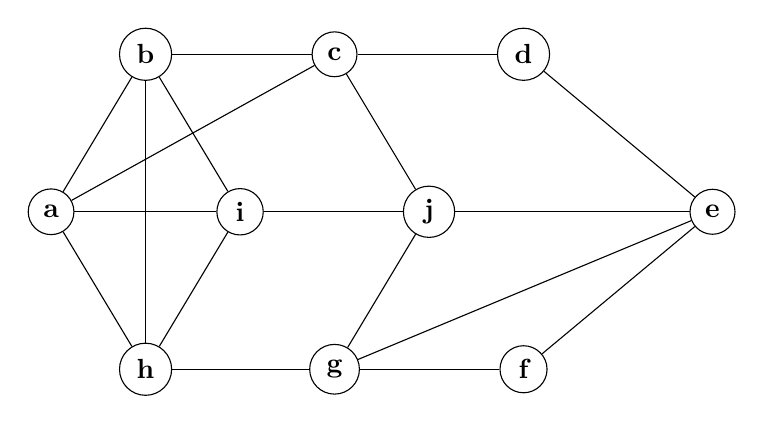
\begin{tikzpicture}[xscale = 0.6, vertice/.style = {fill=white,circle,draw},]

\node[vertice] (A) at (0,0) {{\bf a}};
\node[vertice] (B) at (2,2) {{\bf b}};
\node[vertice] (C) at (6,2) {{\bf c}};
\node[vertice] (D) at (10,2) {{\bf d}};
\node[vertice] (E) at (14,0) {{\bf e}};
\node[vertice] (F) at (10,-2) {{\bf f}};
\node[vertice] (G) at (6,-2) {{\bf g}};
\node[vertice] (H) at (2,-2) {{\bf h}};
\node[vertice] (I) at (4,0) {{\bf i}};
\node[vertice] (J) at (8,0) {{\bf j}};

\draw (A) -- (B);
\draw (A) -- (C);
\draw (A) -- (H);
\draw (A) -- (I);
\draw (B) -- (C);
\draw (B) -- (H);
\draw (B) -- (I);
\draw (D) -- (E);
\draw (D) -- (C);
\draw (E) -- (F);
\draw (E) -- (G);
\draw (E) -- (J);
\draw (F) -- (G);
\draw (G) -- (H);
\draw (H) -- (I);
\draw (I) -- (J);
\draw (J) -- (C);
\draw (J) -- (G);

\end{tikzpicture}
\end{center}

¿es un grafo Euleriano?. En caso afirmativo, encuentra un ciclo euleriano.

\end{ejer}

{\it Solución.-}

% Escribe tu solucion para el ejercicio 1

El grado de todos los nodos es par, por tanto es euleriano.

\begin{center}
	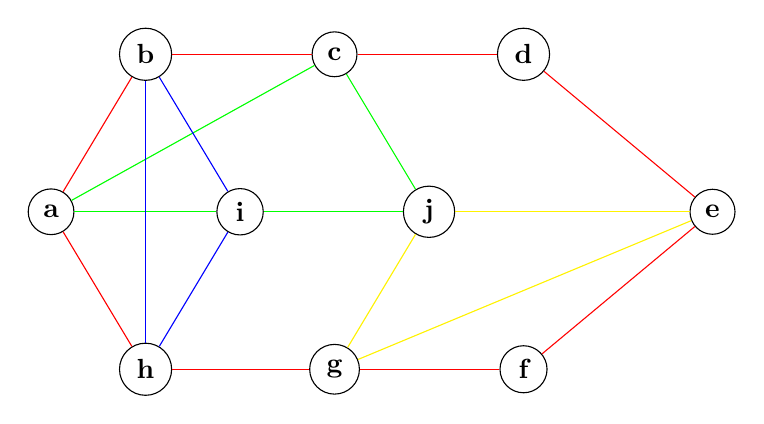
\begin{tikzpicture}[xscale = 0.6, vertice/.style = {fill=white,circle,draw},]
		
		\node[vertice] (A) at (0,0) {{\bf a}};
		\node[vertice] (B) at (2,2) {{\bf b}};
		\node[vertice] (C) at (6,2) {{\bf c}};
		\node[vertice] (D) at (10,2) {{\bf d}};
		\node[vertice] (E) at (14,0) {{\bf e}};
		\node[vertice] (F) at (10,-2) {{\bf f}};
		\node[vertice] (G) at (6,-2) {{\bf g}};
		\node[vertice] (H) at (2,-2) {{\bf h}};
		\node[vertice] (I) at (4,0) {{\bf i}};
		\node[vertice] (J) at (8,0) {{\bf j}};
		
		\draw[draw = red]	(A) -- (B);
		\draw[draw = green] (A) -- (C);
		\draw[draw = red]	(A) -- (H);
		\draw[draw = green] (A) -- (I);
		\draw[draw = red]	(B) -- (C);
		\draw[draw = blue] 	(B) -- (H);
		\draw[draw = blue]	(B) -- (I);
		\draw[draw = red]	(D) -- (E);
		\draw[draw = red]	(D) -- (C);
		\draw[draw = red]	(E) -- (F);
		\draw[draw = yellow](E) -- (G);
		\draw[draw = yellow](E) -- (J);
		\draw[draw = red]	(F) -- (G);
		\draw[draw = red]	(G) -- (H);
		\draw[draw = blue]	(H) -- (I);
		\draw[draw = green] (I) -- (J);
		\draw[draw = green] (J) -- (C);
		\draw[draw = yellow](J) -- (G);
		
	\end{tikzpicture}
\end{center}

\begin{align*}
	{\color{red}(a) - (b) - (c) - (d) - (e) - (f) - (g) - (h) - (a)} \\
	{\color{blue}(b) - (i) - (h) - (b)} \\
	{\color{green}(a) - (c) - (j) - (i) - (a)} \\
	{\color{yellow}(j) - (e) - (g) - (j)}
\end{align*}

$$
	{\color{red}(a) - (b) - (c) - (d) - (e) - (f) - (g) - (h) - (a)} \\
$$

$$
	(a) - {\color{green}(c) - (j) - (i)} - (a) - {\color{red}(b) - (c) - (d) - (e) - (f)} - (g) - {\color{yellow}(j) - (e)} - (g) - (h) - {\color{blue}(b) - (i)} - (h) - (a)
$$

% Fin del ejercicio 1


\begin{ejer}
Dado el grafo ponderado

\begin{center}
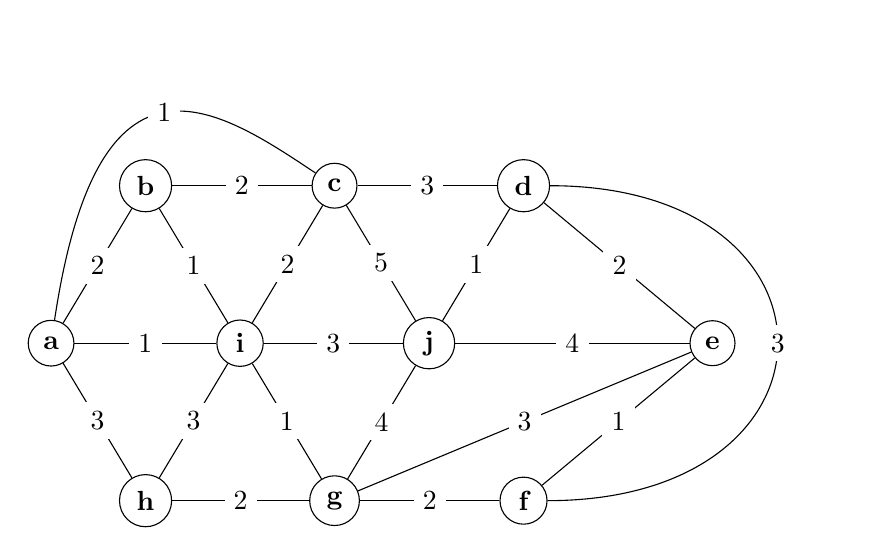
\begin{tikzpicture}[xscale = 0.6, vertice/.style = {fill=white,circle,draw},]

\node[vertice] (A) at (0,0) {{\bf a}};
\node[vertice] (B) at (2,2) {{\bf b}};
\node[vertice] (C) at (6,2) {{\bf c}};
\node[vertice] (D) at (10,2) {{\bf d}};
\node[vertice] (E) at (14,0) {{\bf e}};
\node[vertice] (F) at (10,-2) {{\bf f}};
\node[vertice] (G) at (6,-2) {{\bf g}};
\node[vertice] (H) at (2,-2) {{\bf h}};
\node[vertice] (I) at (4,0) {{\bf i}};
\node[vertice] (J) at (8,0) {{\bf j}};


\draw (A) -- node[fill=white] {2} (B);
\draw (A) .. controls (1,4) and (3.5,3) .. node[fill=white] {1} (C);
\draw (A) -- node[fill=white] {3} (H);
\draw (A) -- node[fill=white] {1} (I);
\draw (B) -- node[fill=white] {2} (C);
\draw (B) -- node[fill=white] {1} (I);
\draw (C) -- node[fill=white] {2} (I);
\draw (D) -- node[fill=white] {2} (E);
\draw (D) -- node[fill=white] {3} (C);
\draw (D) -- node[fill=white] {1} (J);
\draw (D) .. controls (17,2) and (17,-2) .. node[fill=white] {3} (F);
\draw (E) -- node[fill=white] {1} (F);
\draw (E) -- node[fill=white] {3} (G);
\draw (E) -- node[fill=white] {4} (J);
\draw (F) -- node[fill=white] {2} (G);
\draw (G) -- node[fill=white] {2} (H);
\draw (H) -- node[fill=white] {3} (I);
\draw (I) -- node[fill=white] {3} (J);
\draw (G) -- node[fill=white] {1} (I);
\draw (J) -- node[fill=white] {5} (C);
\draw (J) -- node[fill=white] {4} (G);

\end{tikzpicture}
\end{center}

Se pide
\begin{itemize}
\item[a)] Determinar un árbol generador de peso mínimo usando el Algoritmo de Kruskal

\begin{center}
	\begin{tikzpicture}[xscale = 0.6, vertice/.style = {fill=white,circle,draw},]
		\node[vertice] (A) at (0,0) {{\bf a}};
		\node[vertice] (B) at (2,2) {{\bf b}};
		\node[vertice] (C) at (6,2) {{\bf c}};
		\node[vertice] (D) at (10,2) {{\bf d}};
		\node[vertice] (E) at (14,0) {{\bf e}};
		\node[vertice] (F) at (10,-2) {{\bf f}};
		\node[vertice] (G) at (6,-2) {{\bf g}};
		\node[vertice] (H) at (2,-2) {{\bf h}};
		\node[vertice] (I) at (4,0) {{\bf i}};
		\node[vertice] (J) at (8,0) {{\bf j}};
		
		\draw (A) .. controls (1,4) and (3.5,3) .. node[fill=white] {1} (C);
		\draw (A) -- node[fill=white] {1} (I);
		\draw (B) -- node[fill=white] {1} (I);
		\draw (D) -- node[fill=white] {1} (J);
		\draw (E) -- node[fill=white] {1} (F);
		\draw (G) -- node[fill=white] {1} (I);
	\end{tikzpicture}
\end{center}

\begin{center}
	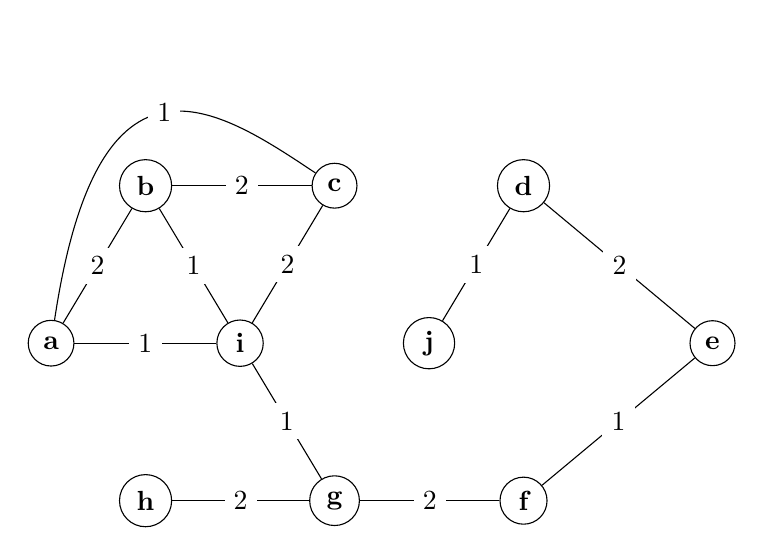
\begin{tikzpicture}[xscale = 0.6, vertice/.style = {fill=white,circle,draw},]
		\node[vertice] (A) at (0,0) {{\bf a}};
		\node[vertice] (B) at (2,2) {{\bf b}};
		\node[vertice] (C) at (6,2) {{\bf c}};
		\node[vertice] (D) at (10,2) {{\bf d}};
		\node[vertice] (E) at (14,0) {{\bf e}};
		\node[vertice] (F) at (10,-2) {{\bf f}};
		\node[vertice] (G) at (6,-2) {{\bf g}};
		\node[vertice] (H) at (2,-2) {{\bf h}};
		\node[vertice] (I) at (4,0) {{\bf i}};
		\node[vertice] (J) at (8,0) {{\bf j}};
		
		\draw (A) -- node[fill=white] {2} (B);
		\draw (A) .. controls (1,4) and (3.5,3) .. node[fill=white] {1} (C);
		\draw (A) -- node[fill=white] {1} (I);
		\draw (B) -- node[fill=white] {2} (C);
		\draw (B) -- node[fill=white] {1} (I);
		\draw (C) -- node[fill=white] {2} (I);
		\draw (D) -- node[fill=white] {2} (E);
		\draw (D) -- node[fill=white] {1} (J);
		\draw (E) -- node[fill=white] {1} (F);
		\draw (F) -- node[fill=white] {2} (G);
		\draw (G) -- node[fill=white] {2} (H);
		\draw (G) -- node[fill=white] {1} (I);
	\end{tikzpicture}
\end{center}

\item[b)] Determinar un árbol generador de peso mínimo usando el Algoritmo de Prim, comenzando por el vértice ${\bf h}$.
\end{itemize}

\end{ejer}

{\it Solución.-}
% Escribe tu solucion para el ejercicio 2

\begin{center}
	\begin{tikzpicture}[xscale = 0.6, vertice/.style = {fill=white,circle,draw},]
		
		\node[vertice] (A) at (0,0) {{\bf a}};
		\node[vertice] (B) at (2,2) {{\bf b}};
		\node[vertice] (C) at (6,2) {{\bf c}};
		\node[vertice] (D) at (10,2) {{\bf d}};
		\node[vertice] (E) at (14,0) {{\bf e}};
		\node[vertice] (F) at (10,-2) {{\bf f}};
		\node[vertice] (G) at (6,-2) {{\bf g}};
		\node[vertice] (H) at (2,-2) {{\bf h}};
		\node[vertice] (I) at (4,0) {{\bf i}};
		\node[vertice] (J) at (8,0) {{\bf j}};
		
		
		\draw (A) .. controls (1,4) and (3.5,3) .. node[fill=white] {1} (C);
		\draw (A) -- node[fill=white] {1} (I);
		\draw (B) -- node[fill=white] {1} (I);
		\draw (D) -- node[fill=white] {2} (E);
		\draw (D) -- node[fill=white] {3} (C);
		\draw (D) -- node[fill=white] {1} (J);
		\draw (E) -- node[fill=white] {1} (F);
		\draw (G) -- node[fill=white] {1} (I);
		\draw (H) -- node[fill=white] {2} (G);
		
	\end{tikzpicture}
\end{center}

% fin del ejercicio 2


\begin{ejer}
Sea el grafo definido por la matriz:

$$\left[
\begin{array}{cccccccccc}
0 & 0 & 0 & 0 & 0 & 0 & 1 & 0 & 0 & 0 \\
0 & 0 & 0 & 0 & 0 & 1 & 1 & 0 & 0 & 0 \\
0 & 0 & 0 & 0 & 0 & 1 & 0 & 1 & 0 & 0 \\
0 & 0 & 0 & 0 & 0 & 0 & 1 & 1 & 1 & 1 \\
0 & 0 & 0 & 0 & 0 & 1 & 0 & 0 & 1 & 1 \\
0 & 1 & 1 & 0 & 1 & 0 & 0 & 0 & 0 & 0 \\
1 & 1 & 0 & 1 & 0 & 0 & 0 & 0 & 0 & 0 \\
0 & 0 & 1 & 1 & 0 & 0 & 0 & 0 & 0 & 0 \\
0 & 0 & 0 & 1 & 1 & 0 & 0 & 0 & 0 & 0 \\
0 & 0 & 0 & 1 & 1 & 0 & 0 & 0 & 0 & 0
\end{array}
\right]
$$
¿ Es un grafo bicoloreable ?. En caso afirmativo obtén una representación bipartita del mismo y encuentra si es posible un emparejamiento.

\end{ejer}

{\it Solución.-}
% Escribe tu solucion para el ejercicio 3

\begin{center}
	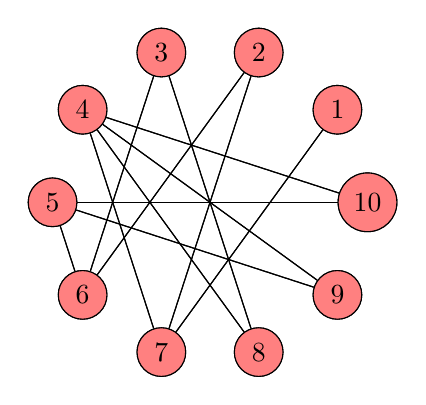
\begin{tikzpicture}[xscale = 1, vertice/.style = {fill=white,circle,draw},azul/.style = {fill=blue!50,circle,draw},rojo/.style = {fill=red!50,circle,draw},]
		\foreach \phi in {1,...,10}{
			\ifthenelse{\phi < 6}{
				\node[azul] (\phi) at (360/10 * \phi:2cm) {\phi};
			}
			{
				\node[rojo] (\phi) at (360/10 * \phi:2cm) {\phi};
			}
			
		}
	
		\draw (7) -- (1);
		\draw (6) -- (2);
		\draw (7) -- (2);
		\draw (6) -- (3);
		\draw (8) -- (3);
		\draw (7) -- (4);
		\draw (8) -- (4);
		\draw (9) -- (4);
		\draw (10) -- (4);
		\draw (6) -- (5);
		\draw (9) -- (5);
		\draw (10) -- (5);
		\draw (2) -- (6);
		\draw (3) -- (6);
		\draw (5) -- (6);
		\draw (1) -- (7);
		\draw (2) -- (7);
		\draw (4) -- (7);
		\draw (3) -- (8);
		\draw (4) -- (8);
		\draw (4) -- (9);
		\draw (5) -- (9);
		\draw (4) -- (10);
		\draw (5) -- (10);
	\end{tikzpicture}
\end{center}

\begin{center}
	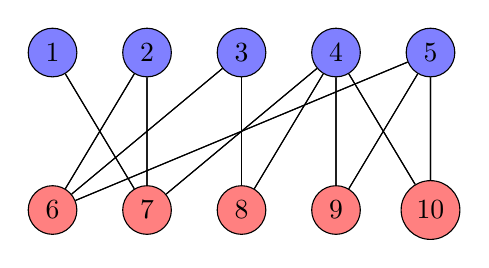
\begin{tikzpicture}[xscale = 0.6, vertice/.style = {fill=white,circle,draw},azul/.style = {fill=blue!50,circle,draw},rojo/.style = {fill=red!50,circle,draw},]
		\node[azul] (1) at (0,2) {1};
		\node[azul] (2) at (2,2) {2};
		\node[azul] (3) at (4,2) {3};
		\node[azul] (4) at (6,2) {4};
		\node[azul] (5) at (8,2) {5};
		\node[rojo] (6) at (0,0) {6};
		\node[rojo] (7) at (2,0) {7};
		\node[rojo] (8) at (4,0) {8};
		\node[rojo] (9) at (6,0) {9};
		\node[rojo] (10) at (8,0) {10};
		
		\draw (7) -- (1);
		\draw (6) -- (2);
		\draw (7) -- (2);
		\draw (6) -- (3);
		\draw (8) -- (3);
		\draw (7) -- (4);
		\draw (8) -- (4);
		\draw (9) -- (4);
		\draw (10) -- (4);
		\draw (6) -- (5);
		\draw (9) -- (5);
		\draw (10) -- (5);
		\draw (2) -- (6);
		\draw (3) -- (6);
		\draw (5) -- (6);
		\draw (1) -- (7);
		\draw (2) -- (7);
		\draw (4) -- (7);
		\draw (3) -- (8);
		\draw (4) -- (8);
		\draw (4) -- (9);
		\draw (5) -- (9);
		\draw (4) -- (10);
		\draw (5) -- (10);
	\end{tikzpicture}
\end{center}

% fin del ejercicio 3



\end{document}


